\begin{figure}[h]
        \centering
        \begin{subfigure}[b]{0.5\textwidth}
                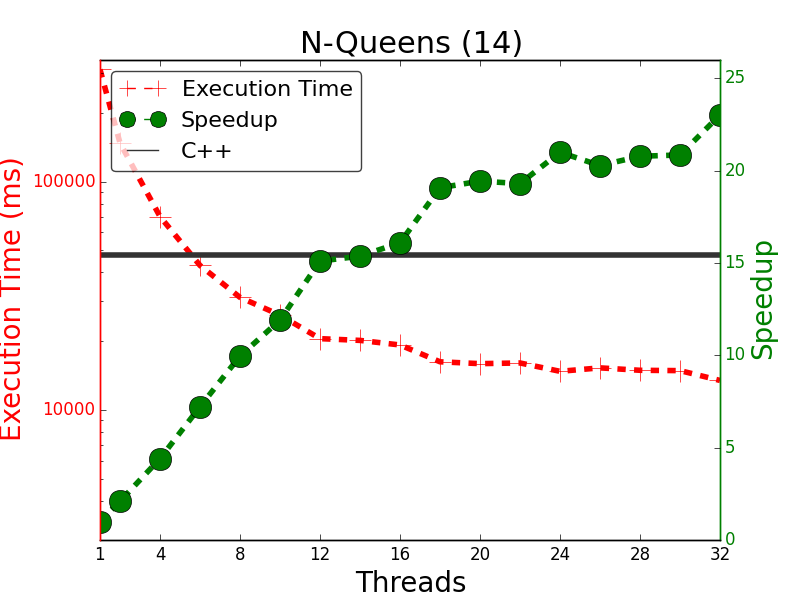
\includegraphics[width=\textwidth]{experiments/scalability/scale-8queens-14.png}
                \label{fig:implementation:scale_queens}
        \end{subfigure}%
        ~
        \begin{subfigure}[b]{0.5\textwidth}
                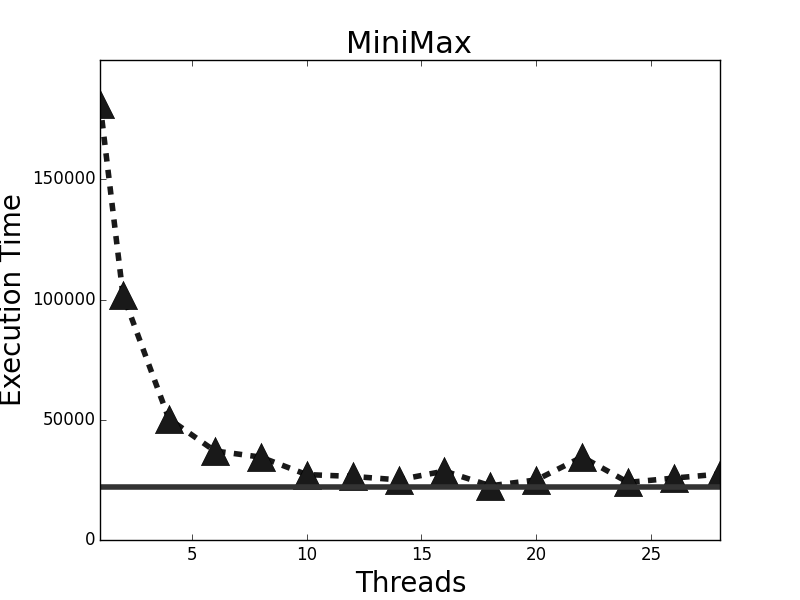
\includegraphics[width=\textwidth]{experiments/scalability/scale-min-max-tictactoe.png}

                \label{fig:implementation:scale_minmax}
        \end{subfigure}\\
        \begin{subfigure}[b]{0.5\textwidth}
                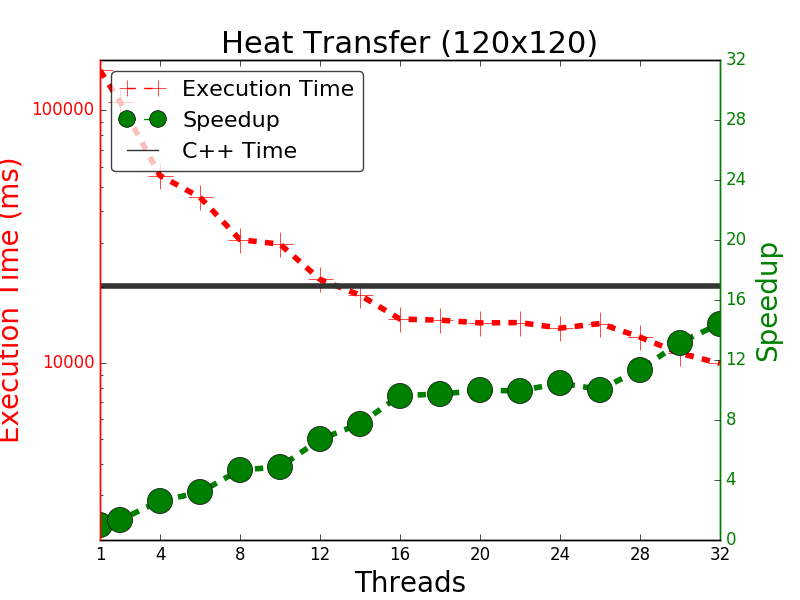
\includegraphics[width=\textwidth]{experiments/scalability/scale-new-heat-transfer-120.png}
                \label{fig:implementation:scale_heat}
        \end{subfigure}%
        ~
        \begin{subfigure}[b]{0.5\textwidth}
                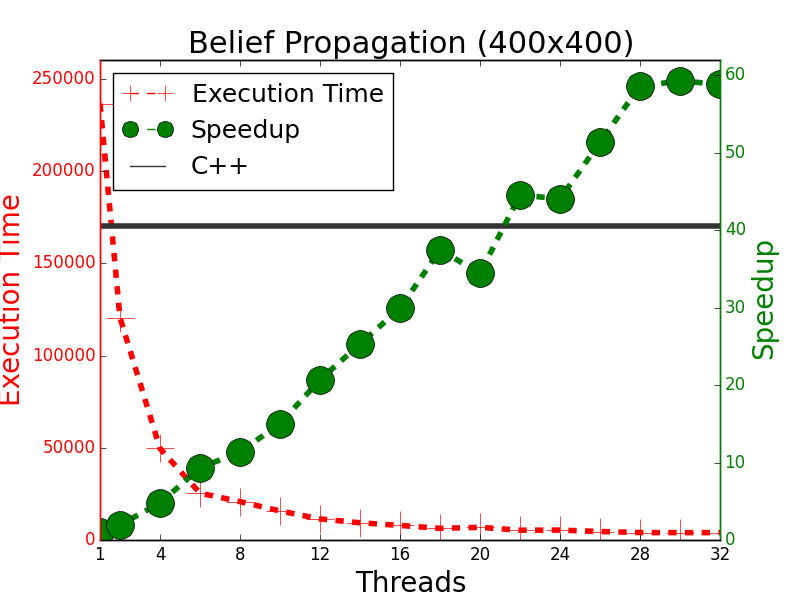
\includegraphics[width=\textwidth]{experiments/scalability/scale-belief-propagation-400.png}

                \label{fig:implementation:scale_bp}
        \end{subfigure}\\
        \caption{An execution trace for the binary tree dictionary
           algorithm. The first argument of each fact was dropped and the
           address of the node was placed beside it.}
        \label{fig:implementation:scale1}
\end{figure}

\begin{figure}[h]
        \centering
        \begin{subfigure}[b]{0.5\textwidth}
                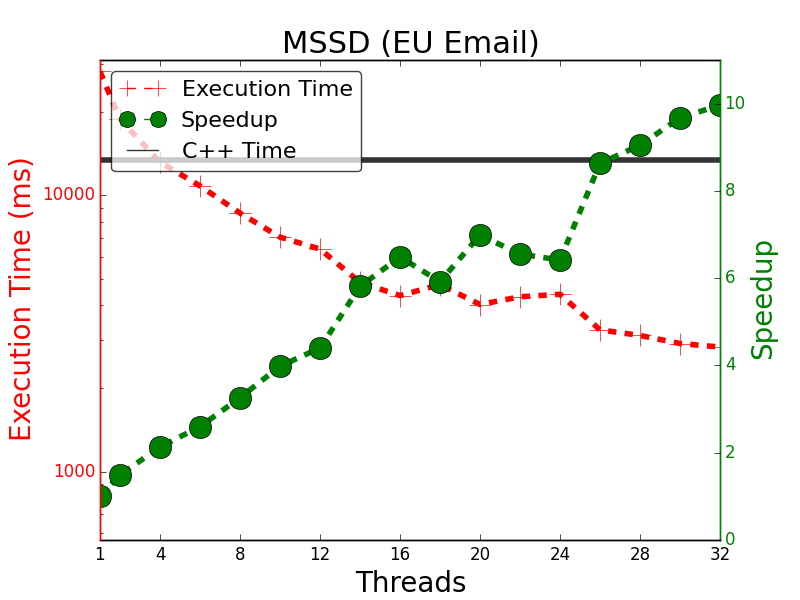
\includegraphics[width=\textwidth]{experiments/scalability/scale-shortest-email.png}
                \label{fig:implementation:scale_sssp_email}
        \end{subfigure}%
        ~
        \begin{subfigure}[b]{0.5\textwidth}
                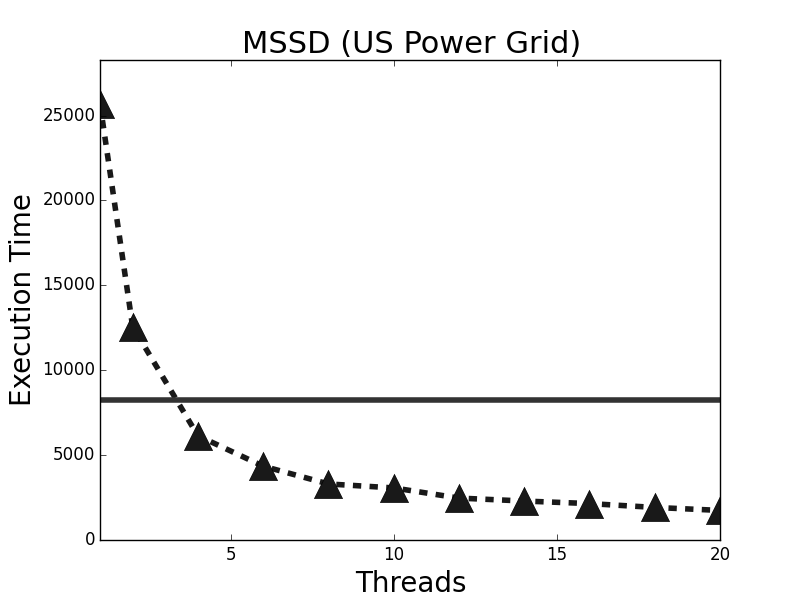
\includegraphics[width=\textwidth]{experiments/scalability/scale-shortest-uspowergrid.png}

                \label{fig:implementation:scale_sssp_uspowergrid}
        \end{subfigure}\\
        \begin{subfigure}[b]{0.5\textwidth}
                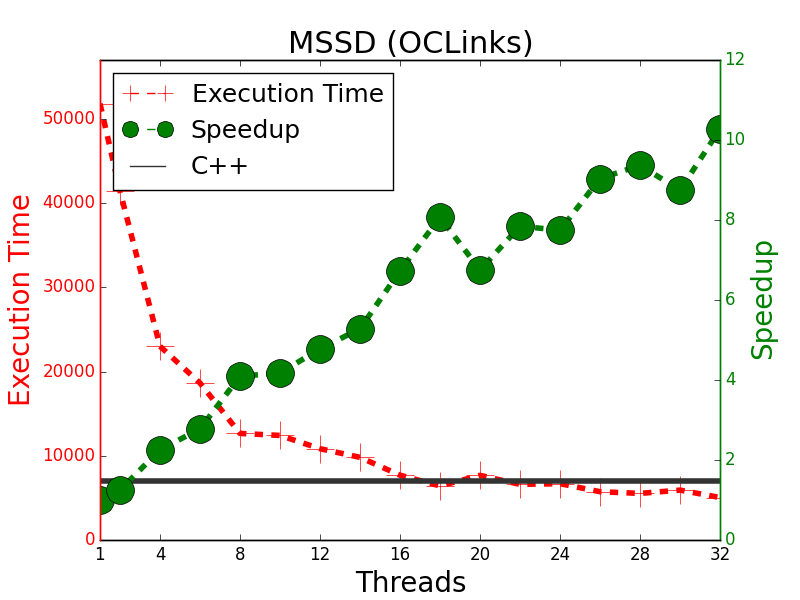
\includegraphics[width=\textwidth]{experiments/scalability/scale-shortest-oclinks.png}
                \label{fig:implementation:scale_sssp_oclinks}
        \end{subfigure}%
        ~
        \begin{subfigure}[b]{0.5\textwidth}
                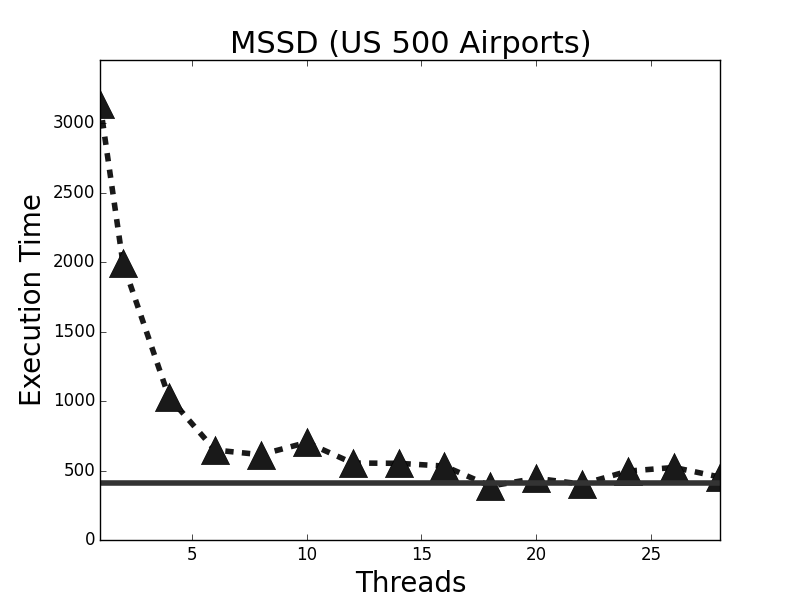
\includegraphics[width=\textwidth]{experiments/scalability/scale-shortest-usairports500.png}

                \label{fig:implementation:scale_sssp_usairports}
        \end{subfigure}\\
        \caption{An execution trace for the binary tree dictionary
           algorithm. The first argument of each fact was dropped and the
           address of the node was placed beside it.}
        \label{fig:implementation:scale2}
\end{figure}
